\documentclass[11pt]{article}

\usepackage{layout}
\usepackage[a4paper, margin=1in]{geometry}
\usepackage{fancyhdr}
\usepackage{amsmath}
\usepackage{amsfonts}
\usepackage{amssymb}

\usepackage[utf8]{inputenc}
\usepackage{algorithm}
\usepackage{algpseudocode}
\usepackage{graphicx}
\usepackage[export]{adjustbox}
\usepackage{titlesec}
\usepackage{setspace}

\pagestyle{fancy}
\lhead{Corinna Lin | 01/25/2023}
\chead{Assignment 1}
\rhead{\thepage}
\setlength{\parindent}{0pt}
\setstretch{1.5}

\begin{document}
Before all questions were attempted, after the respective packages were downloaded, the following commands were run in R:

\begin{verbatim}
    library(ggplot2)
    library(gridExtra)
    library(HistData)
    library(vcd)
\end{verbatim}

\subsection*{1.a) How many rows and columns are in the dataset?}
(For reference, the command \verb|?mpg| was used to answer this question as well as 1.b) \\
The mpg dataset has 234 rows and 11 columns.

\subsection*{1.b) What does the “displ” variable describe?}
The displ variable describes the vehicle's engine displacement, in litres. 

\subsection*{1.c) Which variables are categorical and which are continuous?}
(For reference, the command \verb|?mpg| and \verb|str(mpg)| were used to answer this question) \\
Manufacturer, model, trans, drv, fl, and class are all nominal categorical variables because they do not have an implied order and are categories. Displ, year, cyl, cty, and hwy are all continuous variables because both order and amount are implied.

\subsection*{1.d) Using the ggplot function, make a scatterplot of “displ” against “hwy"}
\begin{verbatim}
    ggplot(data = mpg, mapping = aes(x = displ, y = hwy)) 
    + geom_point(color = "green")
\end{verbatim}

\begin{figure}[H]
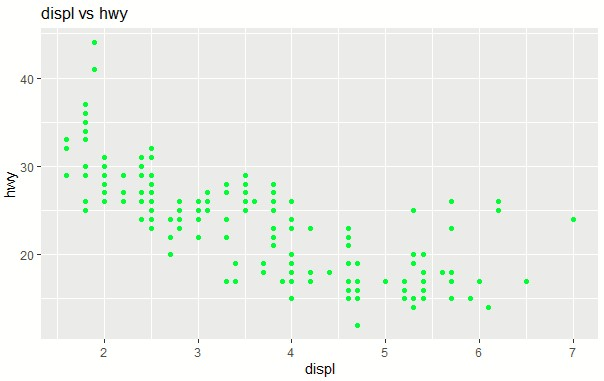
\includegraphics[width = 11cm]{1d.jpg}
\centering
\end{figure}

\subsection*{2.a) Make a histogram displaying “child” height}
\begin{verbatim}
    ggplot(data = Galton, aes(x = child)) + geom_histogram() 
    + labs(title = "Height of Children", x = "Height (cm)", 
    y = "Number of Children")
\end{verbatim}

\begin{figure}[H]
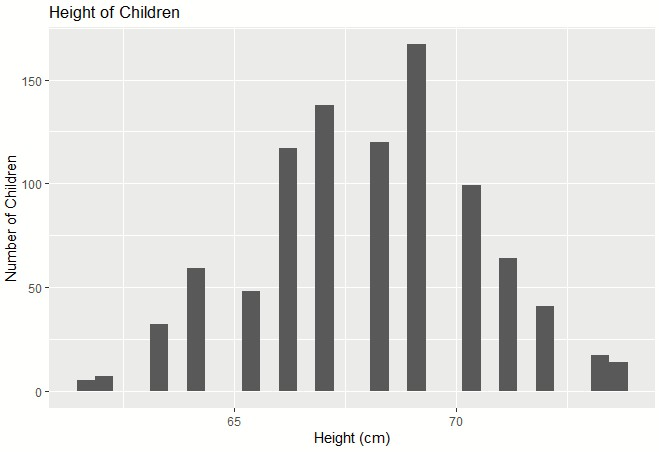
\includegraphics[width = 11cm]{2a.jpg}
\centering
\end{figure}

\subsection*{2.b) Make a histogram displaying “parent” height}
\begin{verbatim}
    ggplot(data = Galton, aes(x = parent)) + geom_histogram() 
    + labs(title = "Height of Parents", x = "Height (cm)",
    y = "Number of Parents")
\end{verbatim}

\begin{figure}[H]
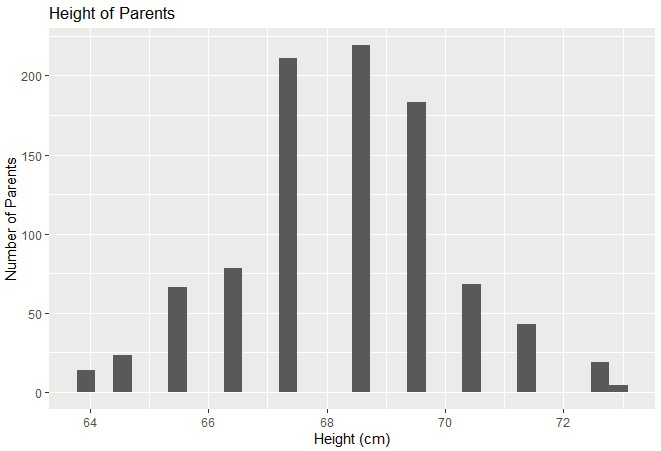
\includegraphics[width = 11cm]{2b.jpg}
\centering
\end{figure}

\subsection*{2.c) Display both graphs in one image}
\begin{verbatim}
    a <- ggplot(data = Galton, aes(x = child)) + geom_histogram() 
    + labs(title = "Height of Children", x = "Height (cm)",
    y = "Number of Children")

    b <- ggplot(data = Galton, aes(x = parent)) + geom_histogram() 
    + labs(title = "Height of Parents", x = "Height (cm)", 
    y = "Number of Parents")

    grid.arrange(a, b)
\end{verbatim}

\begin{figure}[H]
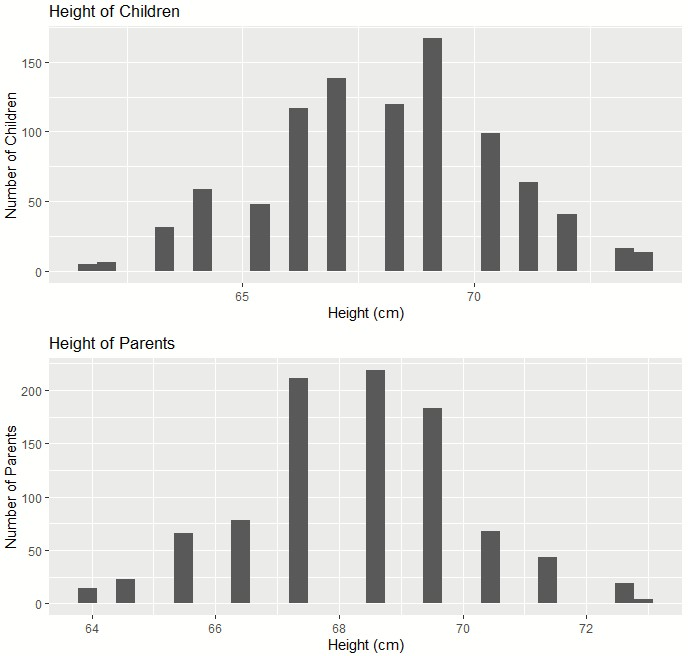
\includegraphics[width = 11cm]{2c.jpg}
\centering
\end{figure}

\subsection*{3.a) Which Vehicle Type has the most observations associated with it in the dataset?}
Suv's have the most observations associated with it in this dataset. The width of this re-scaled stacked and filled bar chart, represents the probability of the data to be in a category. As such, since the width of suv's bar is thicker than the other vehicle types, it occurred most in the dataset and therefore had the most observations.

\subsection*{3.b) For “subcompact” vehicles, what is the majority drive train type?}
For subcompact vehicles, the majority drive train type is f, which is a front wheel drive. The height of this re-scaled stacked and filled bar chart represents the probability of the data to be in each section, which are each identified in the key. In this case, green has the largest area within the subcompact column, which means that f (four wheel drive) had the highest occurrence within subcompact vehicles.

\subsection*{3.c)  For “midsize” vehicles, which of the 3 drive train types occurs least often?}
For midsize vehicles, the drive train type that occurred least often is r, which is a rear wheel drive. This drive train type is represented on the double decker plot in blue, and in the midsize column, the colour that appeared the least is blue, in fact there is no blue in this column (not a single midsized vehicle was a rear wheel drive).

\subsection*{4.a) Create a Double Decker plot, displaying “Age” as a function of “Class” and “Sex”}
\begin{verbatim}
    doubledecker(Age ~ Class + Sex, data = Titanic)
\end{verbatim}

\begin{figure}[H]
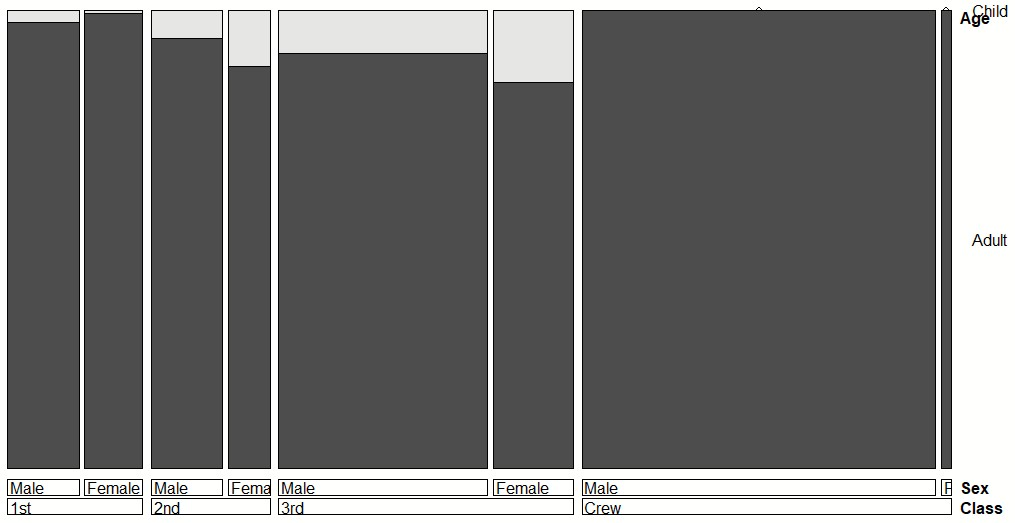
\includegraphics[width = 15cm]{4a.jpg}
\centering
\end{figure}

\newpage

\subsection*{4.b) List 2 interesting facts regarding the observations in the “Crew” Class that the graph shows.}

\begin{itemize}
    \item There were no crew members that were children, they were all adults  
    \item Crew members were male dominant, and there were very few female crew members, I'd say fewer than 5\% were female
\end{itemize}

\subsection*{4.c) The majority of people on board came from which “Class”?}
The majority of people on board came from the crew class, which means they were crew members. On double decker plots, the width of each bar represents the probability of the data to be in a specific category. In this case, when looking at the categories within class, the crew bar has the largest width, which means that within the data, you were more likely to be in the crew class since it occurred most.
\end{document}
